\documentclass[12pt]{article}
\usepackage[utf8]{inputenc}
\usepackage[margin=2cm]{geometry}
\usepackage{amsmath, xcolor, enumitem, graphicx, subcaption, url}
\usepackage[T1]{fontenc}
\usepackage{tgbonum}

\title{\textbf{MA3105: Comparing Cubic Spline with the Linear Spline and the Lagrangian polynomial}}
\author{\emph{Rudra Mukhopadhyay}}
\date{November 24, 2021}

\begin{document}

\maketitle

\tableofcontents

\section{\textcolor{violet}{Aim}}
A counter-intuitive result was noticed after comparing the error in a natural cubic spline to that in a linear spline, for the function $e^x, x\in [-1,1]$. The linear spline error appeared to undergo a faster convergence than the cubic spline, even though the infinity norm error bound in both the cases is given by $\mathcal{O}(h^2), h:=\frac{b-a}{n-1}$ where $n$ is the number of knots in an interval $\Omega = [a,b]$.\\
In this report, I have tried to re-explore the situation and trouble-shoot the set-up. It is examined if the code used contains any manual mistake. An algorithm to estimate the clamped spine, with the first derivative being clamped, has been used.  

\section{\textcolor{violet}{First algorithm in action}}
\subsection{The algorithm given by Atkinson, K. (1978)}
The algorithm used is described briefly underneath.
\begin{enumerate}[itemsep = -4 pt]
    \item $s \in C^2(\Omega)$ be the whole cubic spline on $\Omega$, such that $s = s_{[x_i, x_{i+1}]}$ on $[x_i, x_{i+1}], i = 1, \dots, n-1$.
    \item $\sigma_i := s''(x_i) i = 1, \dots, n$.
    \item $s''$ is linear on $[x_i, x_{i+1}] \implies s''(x) = \dfrac{x_{i+1}-x}{h_i}\sigma_i + \dfrac{x-x_i}{h_i}\sigma_{i+1}, h_i:=x_{i+1}-x_i$.
    \item $s''$ is continuous. Thus, $
    h_{i+1} \sigma_i + 2(h_{i+2} + h_{i+1})\sigma_{i+1} + h_{i+2}\sigma_{i+2} =6\Big(\dfrac{f(x_{i+2})-f(x_{i+1})}{h_{i+2}}-\dfrac{f(x_{i+1})-f(x_i)}{h_{i+1}}\Big), x = 2,\dots ,n-2$. This, along with $\sigma_0 = \sigma_{n} = 0$, constitute the tridiagonal system.
    \item The system of linear equations is solved using Thomas algorithm.
    \item Integrating $s''$ twice yields $s'$ and $s$ respectively.
    \item Using $(i) s' \text{ is continuous}, \text{ }(ii) s \text{ is continuous}, \text{ }(iii) s(x_i) = f(x_i)$ and some algebraic manipulations, an expression for $s(x, \sigma)$ [Ref: Pg 150, Atkinson (3rd ed)] is derived.
    \item Substitute the value of $\sigma_i$ in the expression for $s$.
\end{enumerate}

\subsection{Gauging the accuracy while implementing the algorithm}
\subsubsection{Interpolating a linear function}
On $\Omega = [0,1]$ I have taken {\fontfamily{qcr}\selectfont x = linspace(0, 1, n), y = x}, while {\fontfamily{qcr}\selectfont n = 5:5:30}. The error is presented below.
\begin{table}[h]
    \centering
    \begin{tabular}{|c|c|c|}
    \hline
        n & $||f-s||_\infty$ & $||f -s||_2$ \\
        \hline
        \hline
        5 & 0.000000 & 0.000000\\
        \hline
        10 & 0.000000 & 0.000000\\
        \hline
        15 & 0.000000 & 0.000000\\
        \hline
        20 & 0.000000 & 0.000000\\
        \hline
        25 & 0.000000 & 0.000000\\
        \hline
        30 & 0.000000 & 0.000000\\
        \hline
    \end{tabular}
    \caption{On $\Omega = [0,1], f(x) = x$}
\end{table}
I consider another case, with $\Omega = [100, 120]$, just so that the low error value is not attributed to small {\fontfamily{qcr}\selectfont x(i), y(i)} values.
\begin{table}[h]
    \centering
    \begin{tabular}{|c|c|c|}
    \hline
        n & $||f-s||_\infty$ & $||f -s||_2$ \\
        \hline
        \hline
        5 & 0.000000 & 0.000000\\
        \hline
        10 & 0.000000 & 0.000000\\
        \hline
        15 & 0.000000 & 0.000000\\
        \hline
        20 & 0.000000 & 0.000004\\
        \hline
        25 & 0.000000 & 0.000000\\
        \hline
        30 & 0.000000 & 0.000000\\
        \hline
    \end{tabular}
    \caption{On $\Omega = [100,120], f(x) = x$}
\end{table}
\\It is thus concluded that the program runs accurately for a linear function.

\subsubsection{Comparison with a solved example in Atkinson, 2nd ed}
In this portion, I take under consideration one solved example (Example 4.3.1, page 151) in \emph{An Introduction to Numerical Analysis (2nd ed.)} by Atkinson, K.\\
Given {\fontfamily{qcr}\selectfont x = [1 2 3 4], y = [1 1/2 1/3 1/4]}, it is obvious that the original function $f(x) = \frac{1}{x}, x \in [1,4]$. Using {\fontfamily{qcr}\selectfont n = 4}, I implement the code and report the deviation on the interval $\Omega = [1,4]$. Here $s_1$ represents the spline estimation given by Atkinson, K. and $s_2$ represents the interpolation found by my code.\\
$||s_1-s_2||_\infty = 1.665 \cdot 10^{-15}$\\
$||s_1-s_2||_2 = 6.128 \cdot 10^{-15}$\\
I claim that the error/ deviation of the order $-15$ is solely caused by floating point approximation. Thus, the result obtained by my code agrees with that given by Atkinson, K.

\subsection{Considering $f(x) = e^x$ on $\Omega = [-1, 1]$}
\subsubsection{Interpolation using natural cubic}
I have interpolated the function on $\Omega$, with {\fontfamily{qcr}\selectfont n = 5:5:40}. One instance (with $n = 20$ is plotted.
\begin{figure}[h]
    \centering
    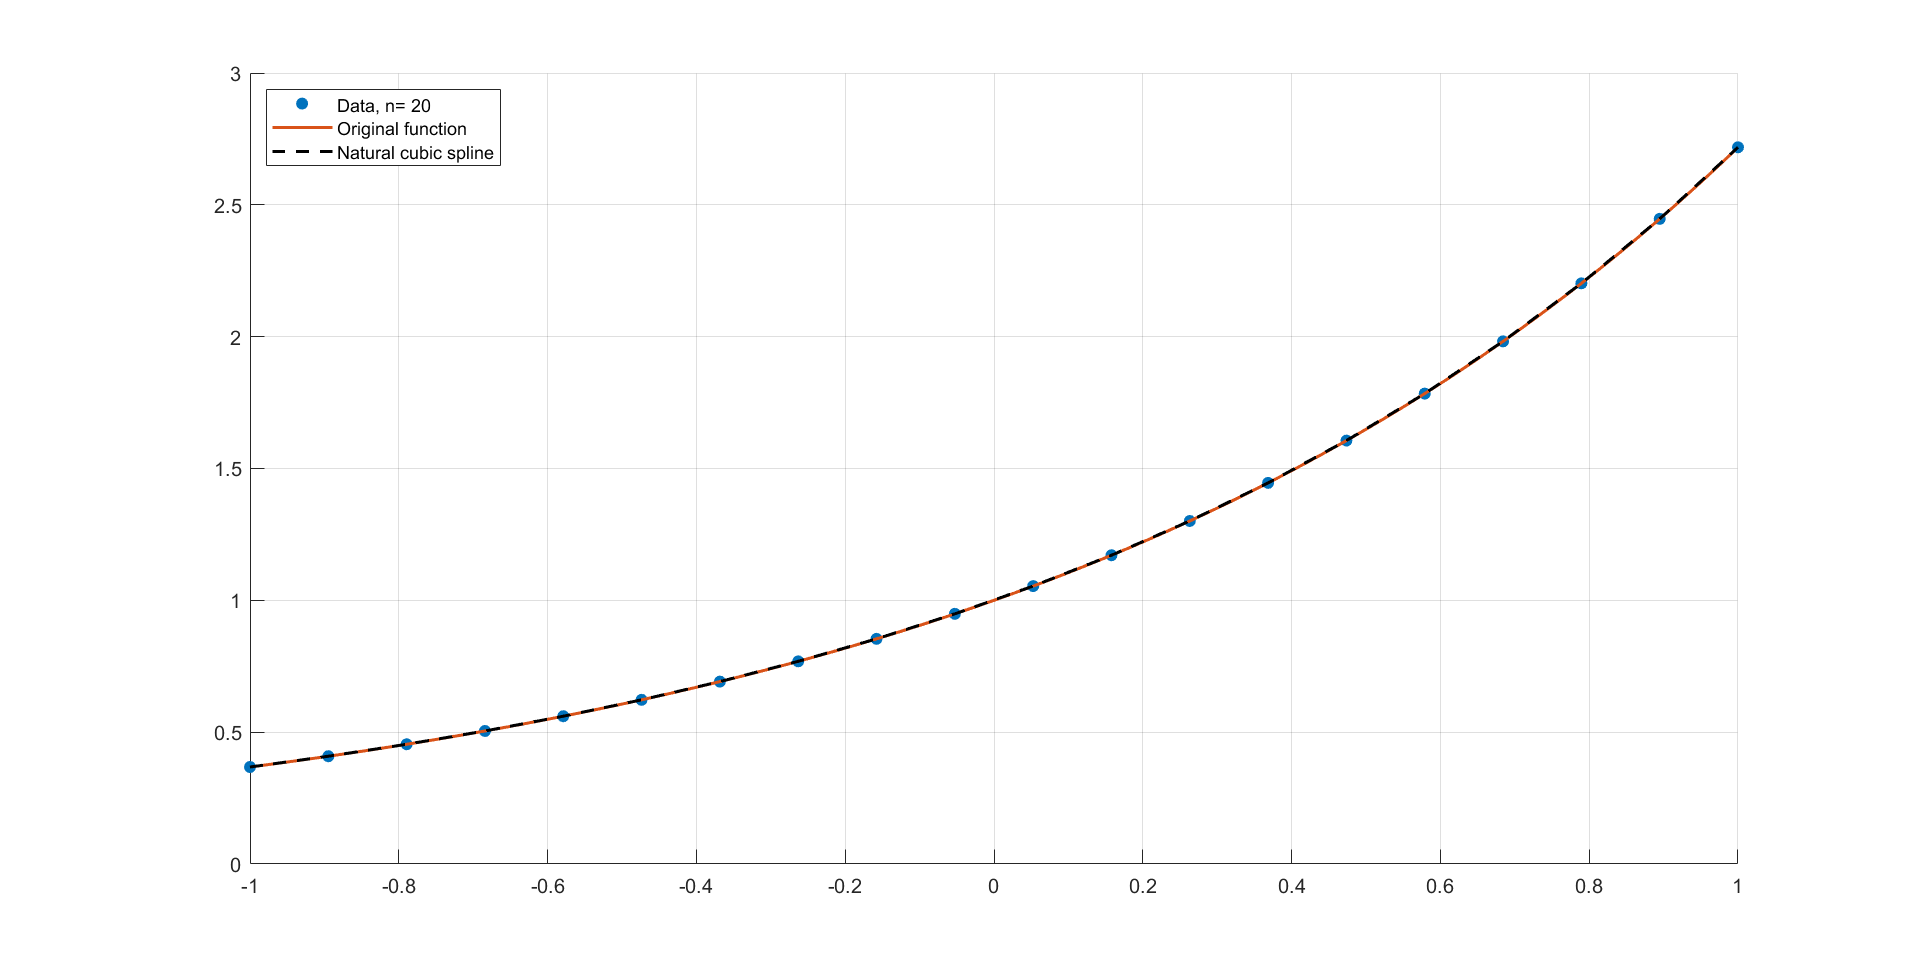
\includegraphics[scale = 0.25]{nat_cub_20.png}
    \caption{Interpolating natural cubic on $\Omega$, for the given $f$}
    \label{fig:my_label}
\end{figure}

\subsubsection{Comparing with the linear spline}
The errors are estimated and presented below. $s_L$ denotes the linear spline, whereas $s_N$ refers to the natural cubic spline.\\
In the second table are presented the ratio $r := \epsilon_{n+1}/\epsilon_n$, where $\epsilon_n$ denotes the error with $n$ number of knots and $\epsilon_n$ is either $L_\infty (r_\infty)$ or $L_2(r_2)$ norm error.
\begin{table}[ht]
    \centering
    \begin{tabular}{|c|c|c|c|c|}
        \hline
        n & $||f-s_L||_\infty$ & $||f-s_N||_\infty$
        & $||f-s_L||_2$ & $||f-s_N||_2$\\
        \hline 
        \hline
        5 & 0.066617 & 0.048949 & 0.428488 & 0.276201\\
        \hline
        10 & 0.015034 & 0.013057 & 0.085609 & 0.069094\\
        \hline
        15 & 0.006460 & 0.005902 & 0.035438 & 0.030806\\
        \hline
        20 & 0.003567 & 0.003340 & 0.019251 & 0.017352\\
        \hline
        25 & 0.002261 & 0.002146 & 0.012068 & 0.011112\\
        \hline
        30 & 0.001537 & 0.001474 & 0.008267 & 0.007720\\
        \hline
        35 & 0.001141 & 0.001099 & 0.006014 & 0.005673\\
        \hline
        40 & 0.000845 & 0.000816 & 0.004571 & 0.004344\\
        \hline
    \end{tabular}
    \caption{Comparing the $L_\infty$ and $L_2$ error}
\end{table}
\begin{table}[h]
    \centering
    \begin{tabular}{|c|c|c|c|c|}
    \hline
        n & $r^L_\infty$ & $r^N_\infty$ & $r^L_2$ & $r^N_2$ \\
        \hline \hline
        10 & 4.430915 & 3.748837 & 5.005196 & 3.997496\\
        \hline
        15 & 2.327467 & 2.212152 & 2.415736 & 2.242852\\
        \hline
        20 & 1.810970 & 1.767133 & 1.840851 & 1.775395\\
        \hline
        25 & 1.577389 & 1.556223 & 1.595191 & 1.561476\\
        \hline
        30 & 1.470864 & 1.455658 & 1.459872 & 1.439444\\
        \hline
        35 & 1.347339 & 1.341709 & 1.374452 & 1.360800\\
        \hline
        40 & 1.350981 & 1.346761 & 1.315722 & 1.305978\\
        \hline
    \end{tabular}
    \caption{Ratio: $||f-s_j||^{n+1}_\rho/||f-s_j||^n_\rho$}
    \label{tab:my_label}
\end{table}

\newpage
As evident from the tables given, the value of error, for both the norms, is lower in the natural cubic spline interpolation. This contradicts the result I showed in the presentation. The mistake most probably lied in the usage of the mesh. Possibly, while calculating the error values, the mesh used in the linear spline case, to estimate the interpolated values, was different from that used in the cubic spline case. Note that, the ratio estimated is similar in both the cases. This can be justified by the fact that linear as well as natural cubic spline has an error bound of $\mathcal{O}(h^2)$.\\
Given below two figures, showing the linear spline, the cubic spline as well as the original function in the same plot.\\
In the second figure, behaviours of these functions are shown over the interval $[0, 0.5]$. While plotting, I have used $n = 5$ in this particular case.

\begin{figure}
\centering
\begin{subfigure}{0.47\textwidth}
    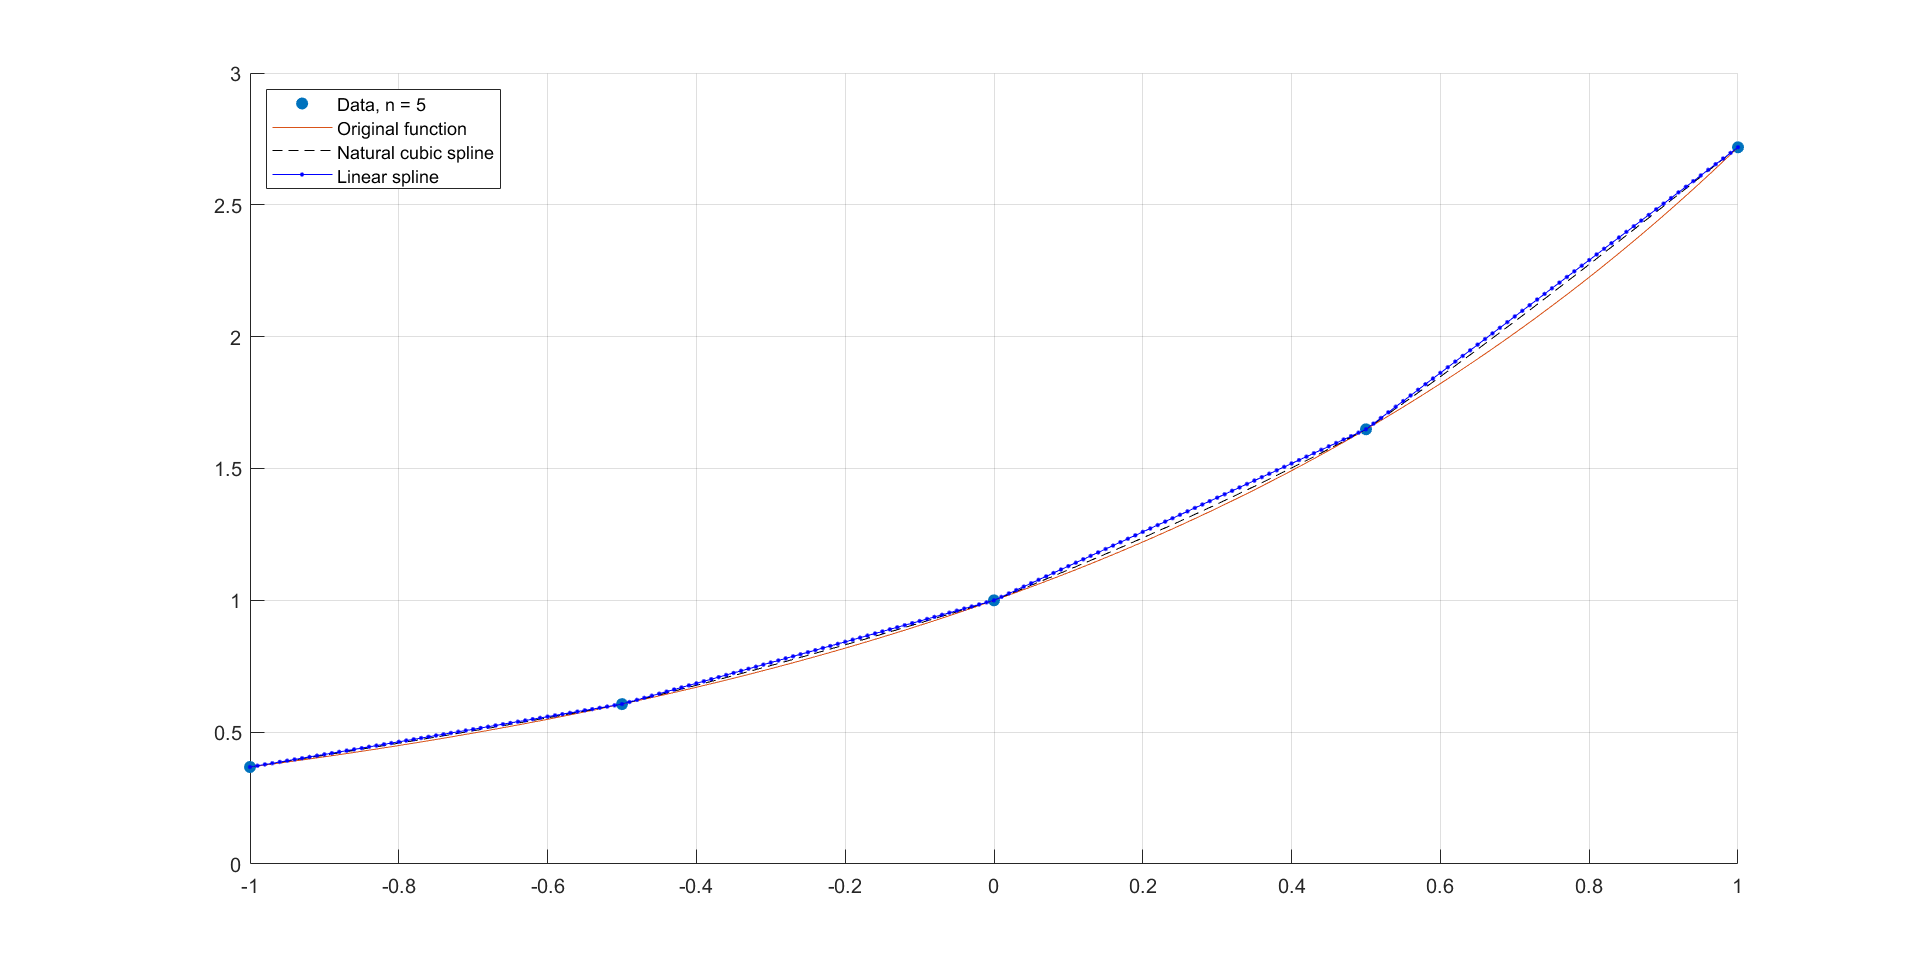
\includegraphics[width=\textwidth]{comp_5_1.png}
\end{subfigure}
\begin{subfigure}{0.47\textwidth}
    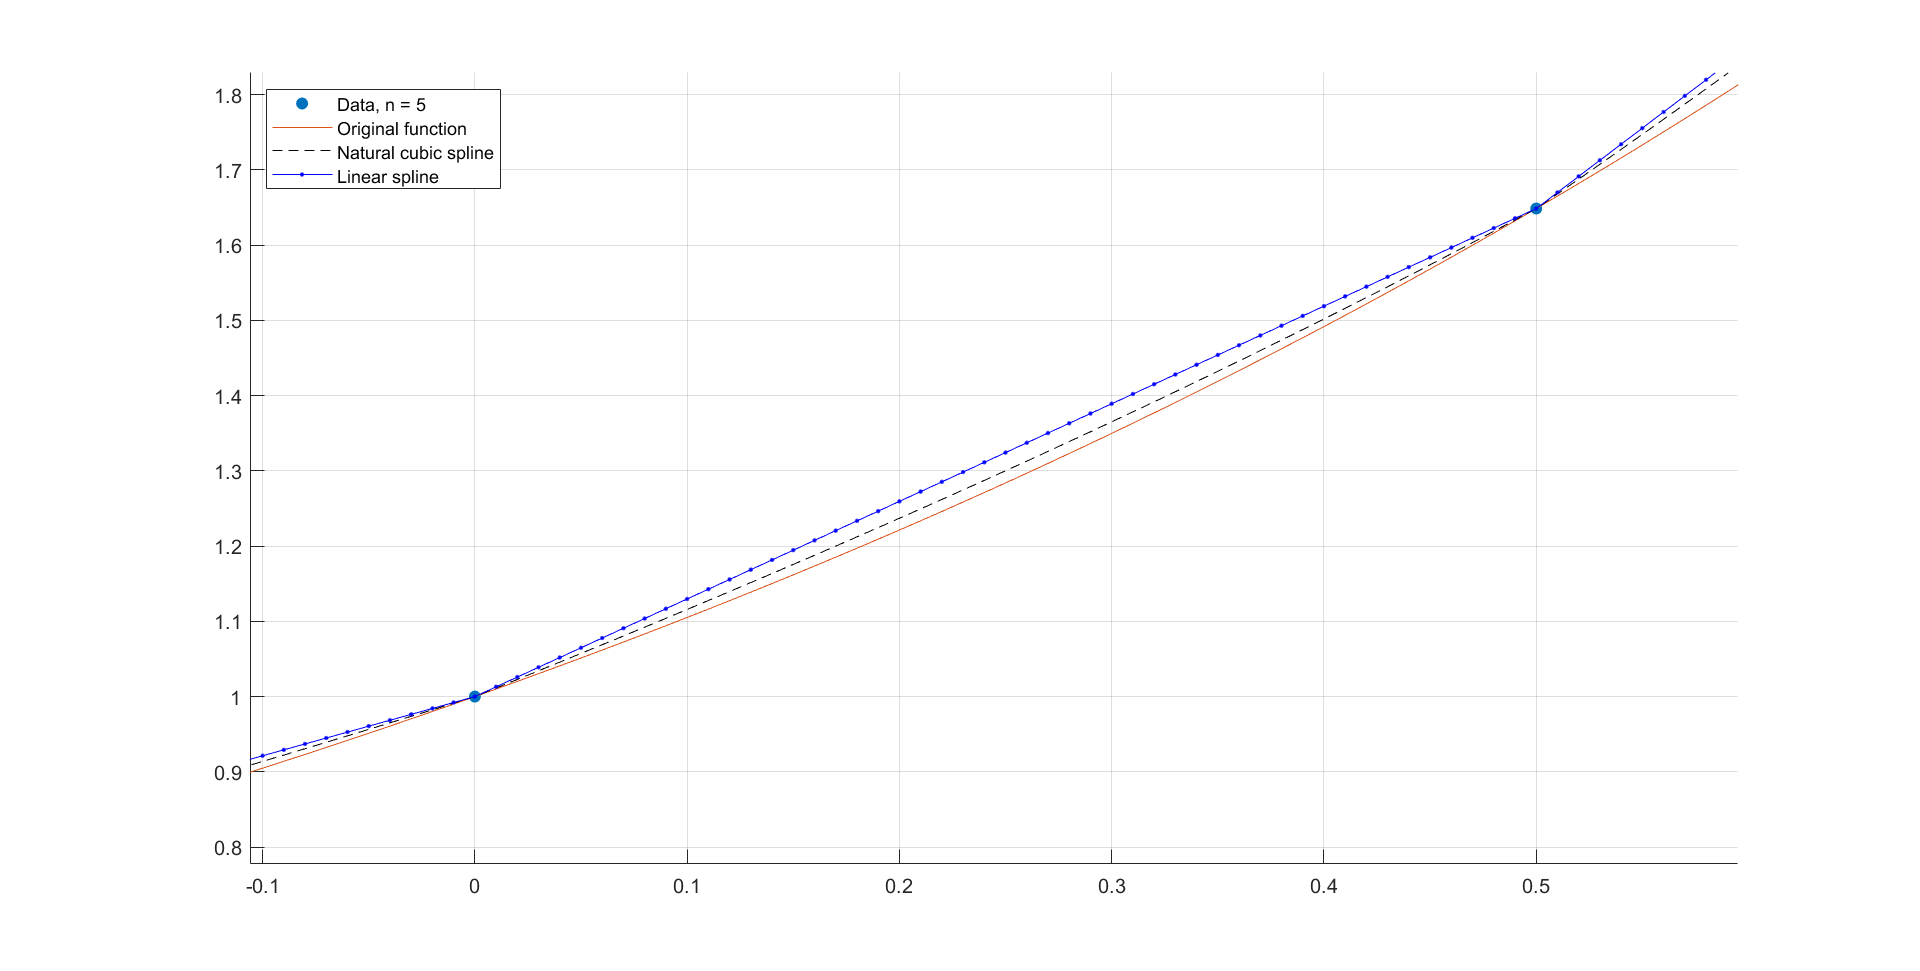
\includegraphics[width=\textwidth]{comp_5_2.png}
\end{subfigure}
        
\caption{Plotting $s_L, s_N \text{ and }, f$}
\end{figure}

\newpage
\section{\textcolor{violet}{Second algorithm in action}}
In the presentation, I presented the clamped condition given by $s''(x_1) = f''(x_1); s''(x_n) = f''(x_n)$. There was no significant improvement in the interpolating spline. Thus, here I discuss the second clamping constraint, given by $s'(x_1) = f'(x_1); s'(x_n) = f'(x_n)$.\\
I have used the algorithm given by Burden, R. and Faires, J. D. in \emph{Numerical Analysis (10th ed.)}. The corresponding Matlab file is uploaded on the GitHub repository mentioned at the bottom of this page  \footnote{\url{https://github.com/MR-dot-15/MA3105-Numerical-Analysis-/blob/main/cubic_spline1.m}}.\\
The error is noted below.
\begin{table}[h]
    \centering
    \begin{tabular}{|c|c|c|c|c|}
        \hline
        n & $||f-s_N||_\infty$ & $||f-s_C||_\infty$
        & $||f-s_N||_2$ & $||f-s_C||_2$\\
        \hline \hline
        5 & 0.048949 & 0.000396 & 0.276201 & 0.002078\\
        \hline
        10 & 0.013057 & 0.000017 & 0.069094 & 0.000078\\
        \hline
        15 & 0.005902 & 0.000003 & 0.030806 & 0.000013\\
        \hline
        20 & 0.003340 & 0.000001 & 0.017352 & 0.000004\\
        \hline
        25 & 0.002146 & 0.000000 & 0.011112 & 0.000002\\
        \hline
        30 & 0.001474 & 0.000000 & 0.007720 & 0.000001\\
        \hline
        35 & 0.001099 & 0.000000 & 0.005673 & 0.000000\\
        \hline
        40 & 0.000816 & 0.000000 & 0.004344 & 0.000000\\
        \hline
    \end{tabular}
    \caption{Comparing natural cubic spline $(s_N)$ with clamped cubic spline $(s_C)$}
\end{table}
\\The fact that the error bound in the clamped cubic is given by $\mathcal{O}(h^4)$ is reflected here, when the first derivative clamping is used. A significant improvement can be noted.\\
A plot containing the natural, clamped cubic spline and the original function is provided below.
\begin{figure}[h]
    \centering
    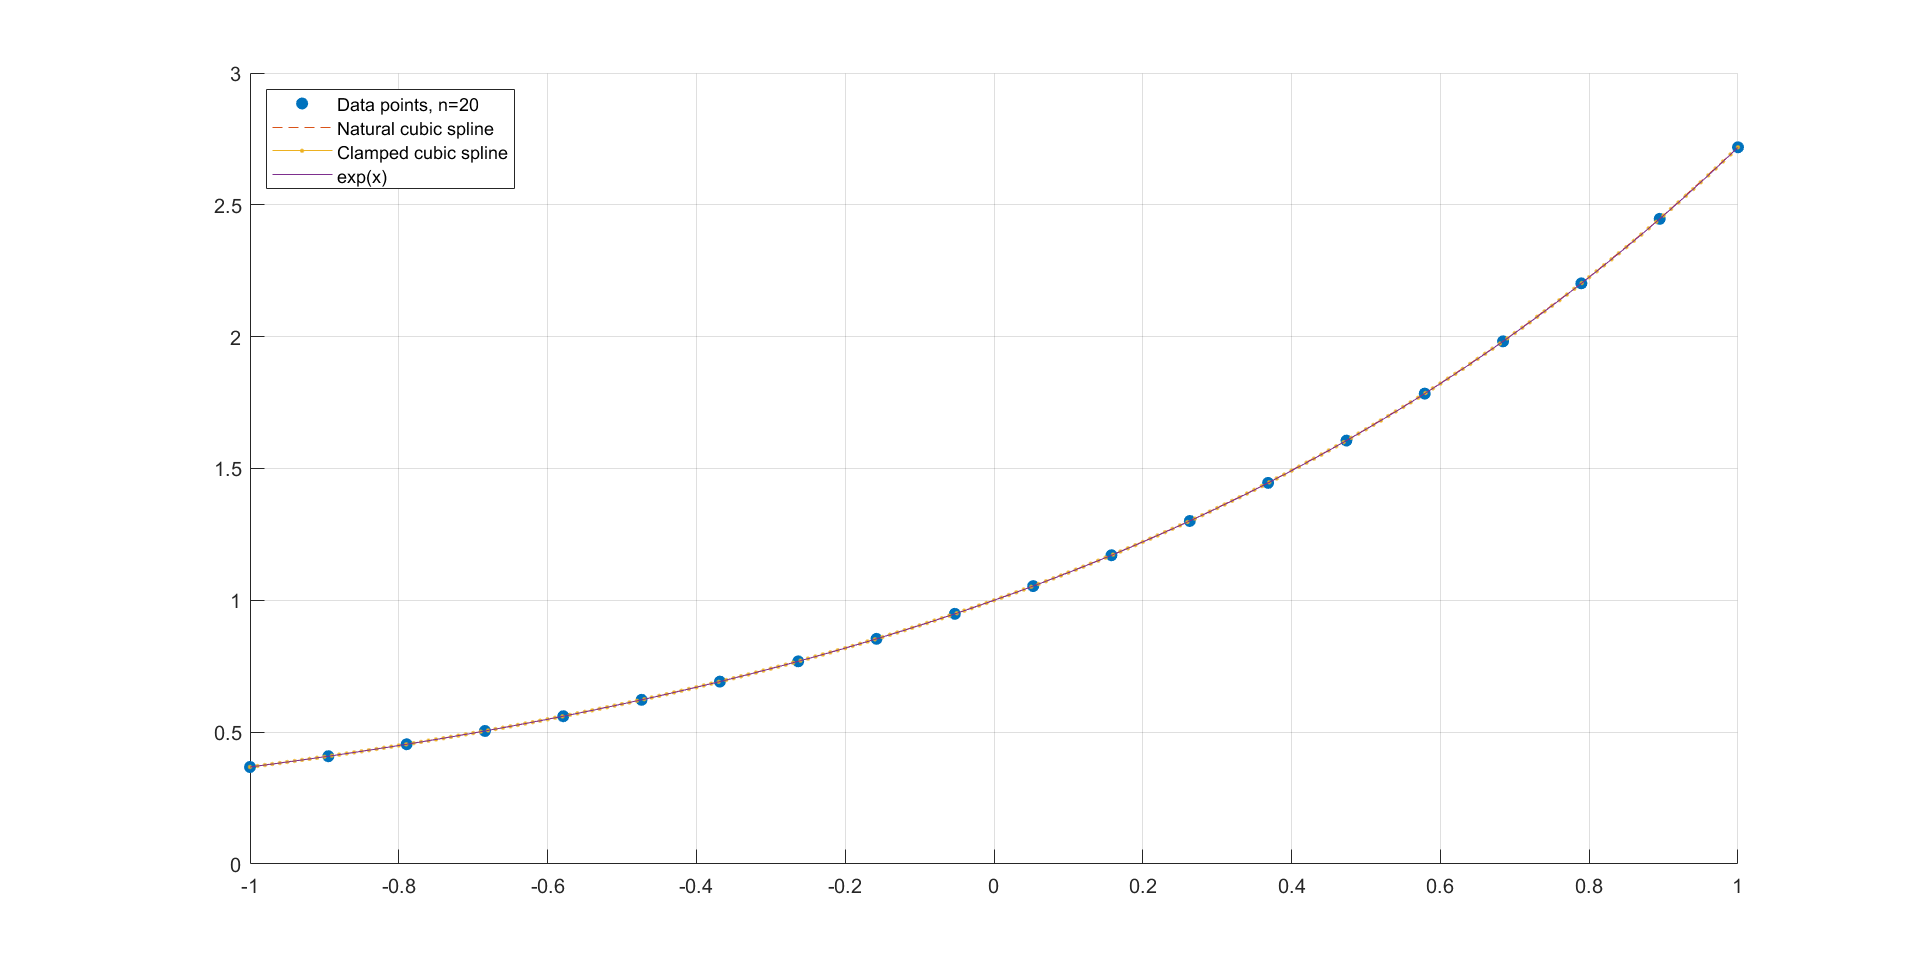
\includegraphics[scale = 0.25]{clmp_nat.png}
    \caption{$s_N, s_C \text{ and } f = e^x$ over $\Omega$. $n=20$.}
\end{figure}

\subsection{Comparing with Lagrangian of degree $n-1$}
In this subsection I have tried to compare the clamped cubic spline with the Lagrangian interpolating polynomial of degree $n-1$. As given by the error bound- $||f-P_n||_\infty \leq \mathcal{O}(h^{n-1})$, a Lagrangian polynomial is supposed to be more accurate than any spline.\\
On the interval $\Omega = [-1,1]$, I estimated $s_C$ and $P_n$, with $n$ varying in $\{4, 6, \dots, 20\}$. While plotting the interpolates, I have used a mesh with $200$ $x$-values on $\Omega$.
\begin{figure}[h]
    \centering
    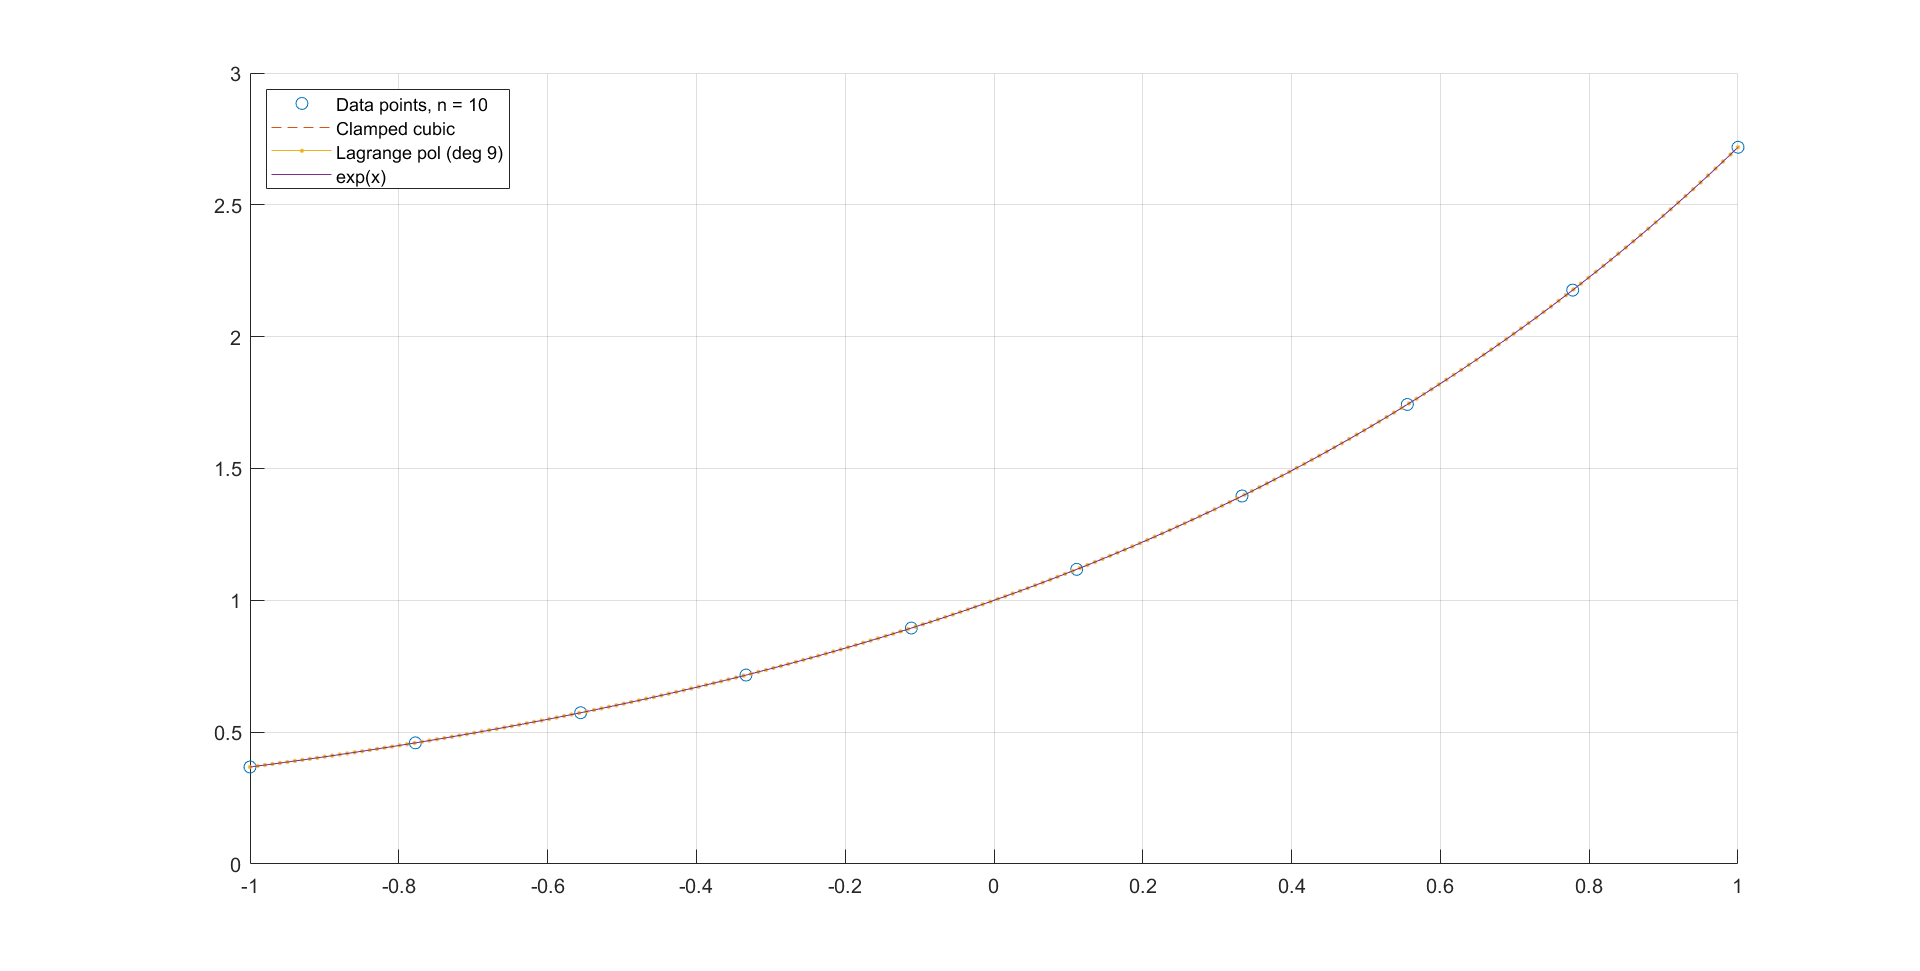
\includegraphics[scale = 0.25]{clmp_lag.png}
    \caption{$s_C, P_n \text{ and } f = e^x$ on $\Omega$}
\end{figure}
\\The error values are presented in the following table.
\begin{table}[h]
    \centering
    \begin{tabular}{|c|c|c|c|c|}
        \hline
        n & $||f-s_C||_\infty$ & $||f-P_n||_\infty$
        & $||f-s_C||_2$ & $||f-P_n||_2$\\
        \hline \hline
        4 & 0.001193 & 0.009983 & 0.006714 & 0.076627\\
        \hline
        6 & 0.000167 & 0.000112 & 0.000835 & 0.000650\\
        \hline
        8 & 0.000045 & 0.000001 & 0.000214 & 0.000004\\
        \hline
        10 & 0.000017 & 0.000000 & 0.000078 & 0.000000\\
        \hline
        12 & 0.000007 & 0.000000 & 0.000035 & 0.000000\\
        \hline
        14 & 0.000004 & 0.000000 & 0.000018 & 0.000000\\
        \hline
        16 & 0.000002 & 0.000000 & 0.000010 & 0.000000\\
        \hline
        18 & 0.000001 & 0.000000 & 0.000006 & 0.000000\\
        \hline
        20 & 0.000001 & 0.000000 & 0.000004 & 0.000000\\
        \hline
    \end{tabular}
    \caption{Comparing the error in clamped cubic spline and the Lagrangian polynomial}
\end{table}
\\As obvious from Table-6, Lagrangian polynomial converges to faster than the clamped cubic. It can be better shown using the ratio of two consecutive errors. 

\subsection{Considering a trigonometric function on $\Omega = [0, \pi]$}
In order to extend the comparison, I consider here the function $f = \sin x$, on the interval $[0, \pi]$. Three different interpolation techniques, namely clamped cubic spline ($s_C$), linear spline ($s_L$) and Lagrangian polynomial ($P_n$) have been implemented. Table-7 contains the infinity and second norm error estimates for all three of those.
\begin{figure}
    \centering
    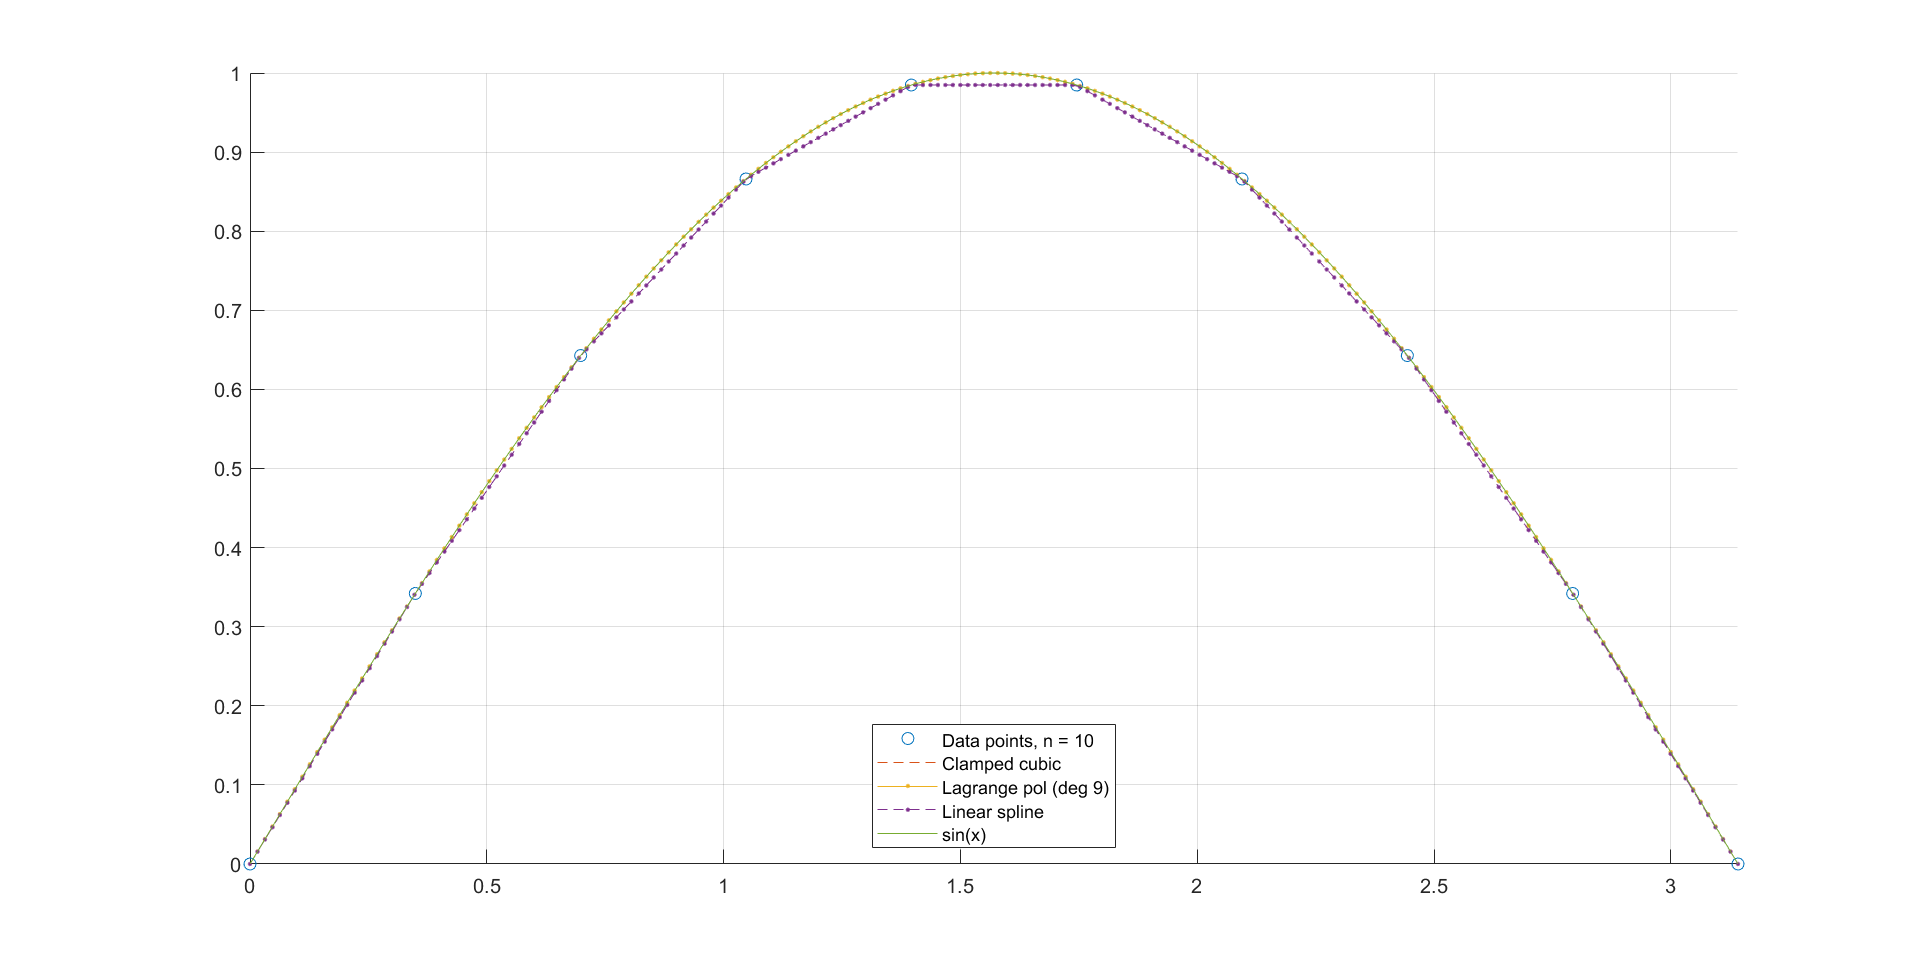
\includegraphics[scale = 0.25]{clmp_lag_sin.png}
    \caption{$s_C, s_L, P_n \text{ and } f = \sin x$ on $\Omega = [0, \pi]$}
\end{figure}
\begin{table}[h]
    \centering
    \begin{tabular}{|c|c|c|c|c|c|c|}
        \hline
        n & $||f-s_C||_\infty$ & $||f-P_n||_\infty$ & $||f-s_L||_\infty$
        & $||f-s_C||_2$ & $||f-P_n||_2$ & $||f-s_L||_2$\\
        \hline \hline
        4 & 0.004733 & 0.043615 & 0.133943 & 0.026204 & 0.385470 & 0.974899\\ 
        \hline 
        6 & 0.000434 & 0.001312 & 0.048912 & 0.002878 & 0.008534 & 0.356398\\ 
        \hline 
        8 & 0.000111 & 0.000024 & 0.025041 & 0.000712 & 0.000127 & 0.182606\\ 
        \hline 
        10 & 0.000040 & 0.000000 & 0.015161 & 0.000255 & 0.000001 & 0.110658\\ 
        \hline 
        12 & 0.000018 & 0.000000 & 0.010147 & 0.000113 & 0.000000 & 0.074142\\ 
        \hline 
        14 & 0.000009 & 0.000000 & 0.007260 & 0.000057 & 0.000000 & 0.053110\\ 
        \hline 
        16 & 0.000005 & 0.000000 & 0.005447 & 0.000032 & 0.000000 & 0.039905\\ 
        \hline 
        18 & 0.000003 & 0.000000 & 0.004235 & 0.000020 & 0.000000 & 0.031074\\ 
        \hline 
        20 & 0.000002 & 0.000000 & 0.003384 & 0.000012 & 0.000000 & 0.024880\\ 
        \hline 
    \end{tabular}
    \caption{Comparing error estimates for $s_C, P_n, s_L$ with $f = \sin x$}
\end{table}

\section{\color{violet}{Conclusion}}
As observed in this analysis, the rate of convergence for both the $L_\infty$ and $L_2$ norm error is the highest when Lagrangian polynomial of degree $n-1$ is used to interpolate $n$ points.\\
It is to be noted that the clamped cubic spline with clamped first derivative yields a better approximation that the natural cubic spline. The accuracy of the linear spline, on the other hand, is \emph{comparable} to that of the natural cubic spline (for both being bounded by $\mathcal{O}(h^2)$). As stated earlier, the result presented showing a significant accuracy in the linear spline case was inaccurate, and was probably caused by using two different set of $x$-values to estimate the interpolated function (i.e. $s_N$ and $s_L$).\\
It can be concluded that, for \emph{significantly large value} of $n$, the approximation accuracy follows this order- Lagrangian polynomial, clamped cubic spline (with the first derivative being constrained), natural cubic spline, linear spline.
\end{document}
